\documentclass[titlepage = firstcover]{scrartcl}
\usepackage[aux]{rerunfilecheck}
\usepackage{fontspec}
\usepackage[main=ngerman, english, french]{babel}

% mehr Pakete hier
\usepackage{expl3}
\usepackage{xparse}

%Mathematik------------------------------------------------------
\usepackage{amsmath}   % unverzichtbare Mathe-Befehle
\usepackage{amssymb}   % viele Mathe-Symbole
\usepackage{mathtools} % Erweiterungen für amsmath
\usepackage[
  math-style=ISO,    % \
  bold-style=ISO,    % |
  sans-style=italic, % | ISO-Standard folgen
  nabla=upright,     % |
  partial=upright,   % /
]{unicode-math}% "Does exactly what it says on the tin."
\usepackage[section, below]{placeins}

% Laden von OTF-Mathefonts
% Ermöglich Unicode Eingabe von Zeichen: α statt \alpha

\setmathfont{Latin Modern Math}
%\setmathfont{Tex Gyre Pagella Math} % alternativ zu Latin Modern Math
\setmathfont{XITS Math}[range={scr, bfscr}]
\setmathfont{XITS Math}[range={cal, bfcal}, StylisticSet=1]

\AtBeginDocument{ % wird bei \begin{document}
  % werden sonst wieder von unicode-math überschrieben
  \RenewDocumentCommand \Re {} {\operatorname{Re}}
  \RenewDocumentCommand \Im {} {\operatorname{Im}}
}
\usepackage{mleftright}
\setlength{\delimitershortfall}{-1sp}

%Sprache----------------------------------------------------------
\usepackage{microtype}
\usepackage{xfrac}
\usepackage[autostyle]{csquotes}    % babel
\usepackage[unicode, pdfusetitle]{hyperref}
\usepackage{bookmark}
\usepackage[shortcuts]{extdash}
%Einstellungen hier, z.B. Fonts
\usepackage{booktabs} % Tabellen


\title{Magnetfelder und Spulen}
\author{
  David Gutnikov\\
  \href{mailto:david.gutnikov@udo.edu}{david.gutnikov@udo.edu}
 \and 
  Lasse Sternemann\\
  \href{mailto:lasse.sternemann@udo.edu}{lasse.sternemann@udo.edu}
}
\date{Durchführung am 03.12.2019}

\begin{document}
    \maketitle
    \newpage
    \tableofcontents
    \newpage

    \section{Zielsetzung}
      Es werden magnetische Flussdichten von Spulen in Abhängigkeit vom Ort gemessen, um sie mit den theoretischen Werten vergleichen zu können. Aus dem
      gleichen Grund wird analog die magnetische Flussdichte eines Spulenpaares in verschiedenen Abständen zueinander gemessen. Außerdem wird mithilfe der
      Hysteresekurve eines Toroides mit Eisenkern seine megnetische Flussdichte, Remanenz, Koerzitivkraft und Sättigungsmagnetisierung gemessen.

    \section{Theoretische Grundlagen}
      Wird eine Ladung bewegt, so wird ein Magnetfeld erzeugt. Dieses Magnetfeld wird durch Magnetfeldlinien dargestellt, welche im Gegensatz zu den
      Feldlinien des elektrischen Feldes immer geschlossen sind. Dabei wird der Betrag und die Richtung des Magnetfeldes entweder durch die magnetische
      Flussdichte $\vec{B}$ oder die magnetische Feldstärke $\vec{H}$ ausgedrückt. Diese beiden Größen sind ohne äußeres Magnetfeld durch die Permeabilität
      $\mu = \mu_0 \cdot \mu_r$, welche sich aus der Vakuum-Permeabilität $\mu_0$ und der relativen Permeabilität in Materie $\mu_r$ zusammensetzt, ineinander
      umwandelbar.
      \begin{equation}
        \vec{B} = \mu \cdot \vec{H}
      \end{equation}
      Fließt ein elektrischer Strom in geraden Leiter, so wird ein Magnetfeld um diesen Leiter erzeugt. Dabei gehen die Feldlinien in Kreisen um den
      Leiter herum. Die magnetische Flussdichte $\text{d}\vec{B}$, die von einem stromdurchflossenen Leiter der Länge $\text{d}\vec{s}$ im Abstand $r$
      erzeugt wird, ist durch das Biot-Savart-Gesetz beschrieben durch:
      \begin{equation}
        \text{d}\vec{B} = \frac{\mu_0 I}{4 \pi} \frac{\text{d}\vec{s} \times \vec{r}}{r^3}
      \end{equation}
      Mithilfe des Biot-Savart-Gesetzes lässt sich die magnetische Flussdichte einer Leiterschleife auf der zur Leiterebene orthogonalen Geraden durch den
      Mittelpunkt bestimmen.
      \begin{equation}
        \vec{B}(x) = \frac{\mu_0 I}{2} \frac{R^2}{(R^2 + x^2)^{3/2}} \cdot \vec{e}_x
      \end{equation}
      \begin{figure}[h]
        \centering
        \caption{Die Skizze der magnetischen Flussdichte einer Leiterschleife. [1]}
        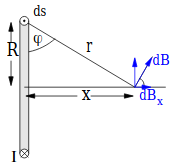
\includegraphics[width = 0.25\linewidth]{Leiterschleife.png}
        \label{fig:leiterschleife}
      \end{figure}
      \FloatBarrier
      Eine Spule mit der Windungszahl $n$ hätte demnach eine um den Faktor $n$ vergrößerte magn. Flussdichte. Ist diese Spule lang, d.h. ihre Länge $L$ ist
      viel größer als ihr Radius $R$, so entsteht im Inneren der Spule ein homogenes Magnetfeld, da die Randeffekte mit steigendem Verhältnis $L/R$ schwächer
      werden. Außerhalb der Spule ist das Magnetfeld inhomogen. Für die magn. Flussdichte innerhalb der langen stromdurchflossenen Spule (Solenoid) gilt dann:
      \begin{equation}
        B = \mu_0 \mu_r \frac{n}{L} I
      \end{equation}
      Werden die beiden Enden eines Solenoides zu einer kreisfprmigen Spule (Toroid) des Umfanges $L = 2 \pi r_\text{T}$ verbunden, so verschwinden die Randeffekte und somit das Magnetfeld
      außerhalb der Spule. Innerhalb der Spule ist das Magnetfeld homogen und es gilt dafür:
      \begin{equation}
        B = \mu_0 \mu_r \frac{n}{2 \pi r_\text{T}} I
      \end{equation}
      Um ein homogenes Magnetfeld zu erzeugen wird oft das sogenannte Helmholz-Spulenpaar verwendet. Es besteht aus zwei Spulen mit gleichem Radius $R$ und
      gleicher Windungszahl $n$, die in gleicher Richtung vom Strom $I$ durchflossen werden und wie in \ref{fig:helmholz} im Abstand von $R$ voneinander entfernt sind.
      \begin{figure}[h]
        \centering
        \caption{Die Skizze eines Helmholz-Spulenpaares. [1]}
        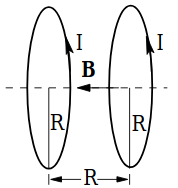
\includegraphics[width = 0.25\linewidth]{Helmholzspulenpaar.png}
        \label{fig:helmholz}
      \end{figure}
      \FloatBarrier
      \noindent
      Das Magnetfeld auf der Symmetrieachse ergibt sich als Überlagerung der Magnetfelder der beiden Spulen:
      \begin{equation}
        \vec{B}(x) = \frac{\mu_0 I n R^2}{(R^2 + x^2)^{3/2}}
      \end{equation}
      Unmagnetisierte ferromagnetische Materialien bestehen aus kleinen magnetischen Momenten, die ohne äußeres Magnetfeld statistisch / "willkürlich" verteilt sind.
      Wird jetzt ein äußeres Magnetfeld angelegt, richten sich diese magn. Momente in Richtung der magn. Feldlinien aus und verstärken das ursprüngliche Mangetfeld.
      Dabei ist die Magnetisierung des Materials irreversibel, weshalb die Magnetisierungskurve (Hysteresekurve) nicht linear ist. Sie fängt bei
      unmagnetisiertem Material im Ursprung bei $B(H=0) = 0$ an und nähert sich mit steigendem angelegten Magnetfeld an einen Sättigungswert $B_r$ an.
      Beim verkleinern des äußeren Magnetfeldes bis auf $H = 0$ bleibt die Remanenz $B_r(H=0) \neq 0$ erhalten. Um diese Restmagnetisierung des Materials
      aufzuheben wird ein anderes Gegenmagnetfeld angelegt, die Koerzitivkraft $H_K$. Wird das Gegenfeld stärker, so wird die Magnetisierung negativ, bis
      sie $-B_r$ erreicht. Hier wird wieder das angelegte Magnetfeld positiver gemacht, was zu einer zum Ursprung punktsymmetrischen Kurve führt.
      \begin{figure}[h]
        \centering
        \caption{Die Skizze einer Hysteresekurve. [1]}
        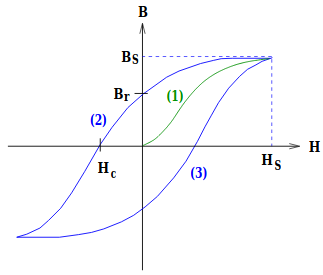
\includegraphics[width = 0.4\linewidth]{Hysteresekurve.png}
        \label{fig:hysterese}
      \end{figure}
      Dabei ist die relative Permeabilität des Materials $\mu_r$ abhängig vom angelegten Magnetfeld $H$ und wird deshalb zur differentiellen Permeabilität $\mu_{\text{diff}}$:
      \begin{equation}
        \mu_{\text{diff}} = \frac{1}{\mu_\text{0}} \frac{\text{d}B}{\text{d}H}
      \end{equation}
      Die magn. Flussdichte einer Spule ist demnach:
      \begin{equation}
        \vec{B} = \mu_0 (\vec{H} + \vec{M})
      \end{equation}

    \section{Durchführung}
      \subsection{Magnetfledmessung einer Spule}
        Hierbei wurden die Magnetfelder zweier verschiedener stromdurchflossener Spulen ausgemessen. Dazu wird eine longitudinale Hall-Sonde parallel in die
        Mitte der Spule eingeführt und die magn. Flussdichte abhängig vom Ort, außerhalb und innerhalb in 1cm Schritten gemessen. Bei ausreichend kurzen Spulen reicht es aus nur von einer Seite aus
        zu messen, doch ist die Spule zu lang kann von zwei Seiten aus gemessen werden, um durchgehend (auch in der Mitte der Spule) Messwerte aufnehmen zu
        können.
      \subsection{Helmholtz-Spulenpaar}
        Hier wird nicht wie bei den klassischen Helmholtzspulen ein Abstand von einem Spulenradius gewählt, sondern es wird der Abstand zwischen den beiden
        stromdurchflossenen Spulen variiert. Es werden drei verschiedene Abstände (10cm, 15cm und 20cm) eingestellt und in Abständen von 1cm mit einer transversalen Hall-Sonde
        ca. 20 Werte der magn. Flussdichte, außerhalb und innerhalb, gemessen. Dabei soll die Hall-Sonde möglichst im rechten Winkel zur Symmetrieachse und
        damit zum Magnetfeld auf der Symmetrieachse.
      \subsection{Hysteresekurve}
        Es ist ein Toroid mit eingebauter Hall-Sonde gegeben, in welchem ein Magnetfeld durch einen angelegten Strom erzeugt wird. Im Anfangszustand sollte
        der Toroid möglichst entmagnetisiert sein, um die Hysteresekurve annähernd aus dem Ursprung starten zu können. Im Verlauf der Messung wird die
        Stromstärke in 1A Schritten bis auf 10A hochgedreht. Danach wird die Stromstärke bis -10A runtergestellt und wieder bis 10A gedreht.
        Dabei entsteht eine Kurve der magn. Flussdichte in Abhängigkeit von der Stromstärke und dadurch der magn. Feldstärke des angelegten Magnetfeldes.



\end{document}